\chapter{Use Cases} \label{sssec:use_cases}

In companies large amounts of data records are retrieved and modified each day. But what if data records are changed or manipulated in a way that the results of your calculations with the data become wrong and decisions are made based on these results? Guaranteeing the integrity of data records in a distributed environment is a big challenge.

This challenge can be tackled by using blockchain technologies. Storing data in the blockchain can guarantee the integrity of your data at all time. Although it gives you many other advantages, storing data, especially large amounts of data, on the blockchain can be very expensive.

The task of this project is to find ways to guarantee the integrity of data stored in a RDBMS with the help of smart contracts. The general idea is to perform integrity checks on data in the smart contract, whenever data is required to perform any transaction. To show the practical relevance of this approach realistic uses cases have to be found and developed. The use cases shall show the potential benefit of storing large amounts of data off-chain but still being able to guarantee the integrity of the data. This is always the case when it comes to financial or personal/contract data.

Throughout the implementation process in this project, we have always been coming up with use cases, and iterate over it to produce a more relateable and complex use cases. The idea is to generate simple uses cases first, apply these to the current prototype implementation, test them in terms of performance and efficiency and show ways to further develop the use cases as well as apply different integrity mechanisms based on the results of the tests.

In the end, we have come up with two different use cases, produced through our feedback sessions and discussions as a group. The uses cases should represent a real case scenario and highlight the need for off-chaining data.

The following points should summarize the properties of our use cases. As mentioned before, the developed uses cases should still be feasible and integratable with the current prototype implementation. 

\begin{itemize}
	\item Multiple Columns:
	In order to make use of the hash tree algorithm a data table with multiple columns is required.
	\item One table per Use Case:
	In the current project stage, the Use Cases should use only one table each. Multiple entities and relations would make the Use Case too complex. In the future, a more complex Use Case with multiple entities and relations could be developed.
	\item Big Data:
	In real world examples large numbers of data records are stored and evaluated every day. Our use cases should consider real world examples, where a large amount of data is required. With the current prototype implementation and the posed constraints by the Ethereum network, a large number of data records could hit the gas limit very quickly. Therefore, the number of data records should be limited to a defined number.
	\item Different Scenarios:
	For presentation purposes, the two use cases should not only use different data types but also do different things with the acquired data. 
\end{itemize}

\subsubsection{Employee Use Case}
\paragraph{Concept - Employee Payraise}
\subparagraph{Description}
In a real world scenario, a company could decide to use the blockchain and the off-chaining approach to verify employee data, which is stored in a private database (RDBMS). Additionally the company wants to make the changes in salaries for each employee as transparent as possible. Together with a union the company can agree on details (e.g. percentage of pay raise, affected departments, etc.) for a pay raise increase and store as well as execute the pay raise on the blockchain.

The general idea to implement this use case is to create two separate Smart Contracts: The employee contract and the pay-raise contract. In the employee contract, we need to store the root hashes, which can be used to verify the integrity of employee data record. The details of pay raise agreed together with company and union are stored in a separate contract called the pay raise contract. When performing the pay raise, the employee contract should be addressed which in turn should address the pay raise contract to extract the details for the pay raise.


\textit{Example: A Employees Table}
\begin{center}
    \begin{tabular}{| l | l | l | l | l |}
    \hline
    RecordID & FirstName & LastName & StartDate & Salary \\ \hline
    1 & Max & Mustermann & 20171230 & 45500 \\ \hline
    ... & ... & ... & ... & ... \\ \hline
    \end{tabular}
\end{center}

As mentioned before the Employee Smart Contract stores the root hashes of each employee record. The table above shows an example Employee table with one record. The merkle tree is constructed with the values in 'FirstName', 'LastName', 'EntryDate' and 'Salary' in the given record. The root of constructed merkle tree is stored in a map with the 'RecordID' as an identifier for the root hash.

\paragraph{Implementation}
\subparagraph{Overview}

\begin{figure}[h]%evtl:[t] [!htbp]
\centering
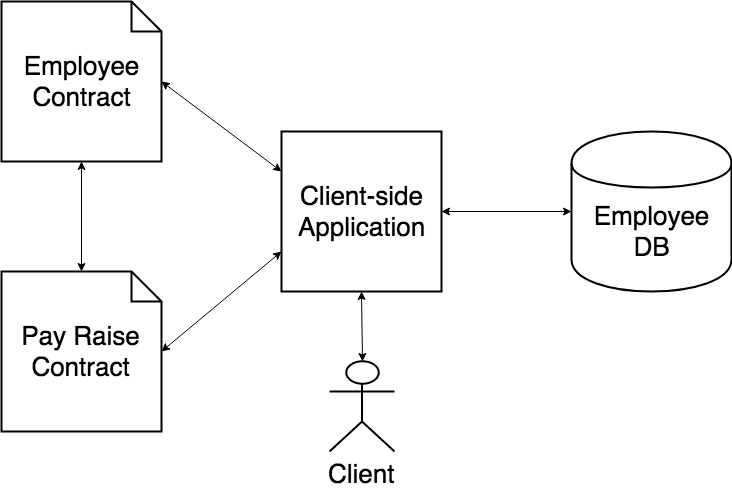
\includegraphics[width=1.0\textwidth]{images/payraiseusecase.png}
\caption{\label{fig:payraiseusecase}Overview of all components of the Employee Use Case}
\end{figure}

As mentioned in the previous chapter, this use case requires two smart contracts, which should interact with each other. Figure \ref{fig:payraiseusecase} shows all the components of this use case and how they interact with each other. In this use case, we have the following components: Client, Client-side Application, Employee DB, Pay Raise Contract and Employee Contract.

The client is basically the user, which is interacting with the whole system. It triggers functions to the client-side application to perform transactions. Applied to the use case, the client can be either the company or the union.

The client-side application is the main part of this use case. It is connected with the employee database, where the employee data is stored in a employee table. By using the Web3 API it is able to create and interact with the employee contract as well as the pay raise contract.

Both contracts, employee contract as well as pay raise contract can exist on their own. But only one employee contact should be created for this uses case. Everytime data is inserted or updated in the employee database, the employee contract is updated accordingly. E.g. when a record is inserted in the database, an additional mapping item with the identifier and the Merkle root of the Merkle tree constructed from this record is inserted into the contract. In case a record is updated, a new Merkle tree has to be constructed in the client-side application and the new Merkle root has to be used to replace the old Merkle root in the equivalent mapping item.


\subparagraph{Necessary Steps}

This subchapter briefly describes the necessary steps for a client to interact with the components in the use case. Also it gives some insights on how the components interact with each other.

\begin{enumerate}
\item Create Employee Contract
\end{enumerate}

In order to perform further transactions, an employee contract has to be created. Via REST interface, the client shall call a function to create a contract. The client-side application takes the request and creates the contract in the network as well as a contract instance inside the application with the contract address, to perform further transactions with the employee contract.

\begin{enumerate}[resume]
\item Create/Import Employee Data
\end{enumerate}

The client can now create data records or use the import function, to create multiple employee data records. The client-side application uses the input of the client to create data records in the employee table in the database. Moreover, it creates for each new employee record a Merkle tree and adds a mapping item with the Merkle root and the “record id” of the employee in the database into the smart contract. 

\begin{enumerate}[resume]
\item Create Pay Raise Contract
\end{enumerate}

Before a pay raise can be executed to employees, specific conditions have to be formulated, for example the percentage, the affected department, etc. Those conditions are formulated in the Pay Raise Contract. This contract contains only the formulated and agreed conditions between the company and the union, as well as getter functions to retrieve these conditions later from the Employee Contract, where the pay raise is executed.

\begin{enumerate}[resume]
\item Increase Salary
\end{enumerate}

In the Increase Salary step, the client triggers a function on the client-side application to increase the salary of all affected employees according to the created pay raise contract in step 3. Therefore the client sends a request with the contract address of the pay raise contract. The client-side application calls a function in the employee contract by passing the pay raise contract as input parameter. After that the employee contract retrieves the conditions (e.g. percentage, department, etc.) from the pay raise contract and returns it to the client-side application as an event. The client-side application listens to this event and uses the conditions as query parameters when querying the database. For example, if the department is ‘IT’, the SQL Query would look like this:

\begin{lstlisting}[language=bash]
SELECT *
FROM Employee
WHERE Department = 'IT'
\end{lstlisting}

For each single employee in the output of the query, a single smart contract transaction is required to increase the salary of the employee. If for example, the number of employees in the IT department is three, then the whole transaction needs additional three smart contract transactions. These three smart contract transactions are chained, meaning they need to be executed sequentially. The reason for that is because the employee contract will send data back to the client-side application via an event. The design decision was to shut down the event listener in the client-side application after it listened to one event. Triggering three smart contract transactions would result in three different events as result for each transaction. Triggering all three smart contract transaction at once would mean that the client-side application would only listen to one event and the whole transaction cannot be completed.

As first step of one smart contract transaction for increasing one single employee, the client-side application calls a smart contract function and sends the whole data record of the employee in the database table as well as the Merkle proofs of the salary of the single employee as input parameters to the smart contract. In the smart contract the integrity of the employee data record is checked. The Merkle root can be retrieved from the mapping item with the record identifier and the Merkle root stored in the smart contract. With the Merkle proof and the hash of the salary of the employee the Merkle root can be constructed. If the constructed Merkle root is the same as the saved Merkle root for the employee record, the integrity check was successful. The salary is then increased by the percentage stored in the pay raise contract. A new Merkle root is constructed out of the new salary and the proofs, which is then stored into the mapping item and sent back as an event to the client-side application together with the new value of the salary. The client-side application takes the new value for the salary of the employee and stores it into to the database. Subsequently, it will continue making a new smart contract transaction for the next employee pay raise. The whole transaction is finished when all employees in the query result are processed.

In case the integrity check fails, the smart contract will send an event to notify the client-side application about the failure. Even if one integrity check of an employee fails, the other employees are still processed. As end result the client will receive as response all employees, whose salary has been increased.

\subparagraph{Discussions}

In this use case the client-side application needs to trust the database to return the correct results. For example if there are actual five people working in the IT department, the database should return the records of those five employees. In this case we are putting some trust in the database to return all those five employees. However,the database could be manipulated by an administrator, such that one or more employees from the IT department are missing in the query result. As a result a pay raise would not affect those missing employees. A possible solution would be to store the number of employees for each department in the smart contract and check whether the number of query results matches with the number of employees for a specific department stored in the smart contract.

\section{Financials}

\subsection{Concept}
\subparagraph{Description}
An external auditor wants to check the financial situation of a company. One task could be to check the stated weekly or monthly sales amount against the sum of all sales records in the specific year. One of the first steps would be to verify (check the integrity) of all sales records in the specific year.

This use case consists of two parties, a financial auditor and the company that holds the financial data. An assumption that we make is that the middleware is open-sourced, produced by an auditing company, and it is being consumed by the company to store their financial data in the blockchain environment. The middleware allows the company to off-chain their financial records from the smart contract into a database, while maintaining the integrity of the data using the blockchain environment. The middleware also allows the auditor to easily audit companies’ financial records without having to worry about the integrity of data once they are appended. It also allows the auditor to query the financial records with a filter, such as the date of the records, performing query completeness. The middleware however does not allow users to edit the records through the middleware, though it is possible to do it on the database directly, which will then result in an integrity check error when the records are used or verified by the auditor.


\begin{table}
	\centering
	\caption{An Example of a Sales Table}
    \begin{tabular}{| l | l | l | l | l |}
    \hline
    ID & Product & Date & Amount & Price \\ \hline
    1 & Wallet & 20171230 & 1 & 20 \\ \hline
    .. & ... & .... & .. & ... \\ \hline
    \end{tabular}
\end{table}

The different table rows represent moments in time (e.g. every Friday night after 00:00 or every first of the month) and thus new records are appended to the table. In this way, the records can be tracked back in time and an auditor could double-check the records for e.g. the last 6 months or the last 104 weeks. The smart contract entry then consists of the root hash over every table row (with each column being a leaf in the Merkle tree).

As the database is under the control of the company storing their financial figures, the financial auditor cannot be sure that those numbers were inserted correctly (same as without blockchain). By having the hashes of the records on the blockchain, the auditor can be sure that the company was not able to change the figures later on and thus has the certainty that there are no accounting tricks and malpractices in place e.g. at the end of the year or quarter. The figures that were once recorded by the company can be double-checked afterwards (or it can be noticed that the company recorded wrong numbers or tried to change them in hindsight). It is worth mentioning that the smart contract never stores the financial figures and they are thus not available on the blockchain either. While upon insertion, there isn’t a way to check that the numbers are true, but we can assert that these numbers will not be prone to illegitimate changes.

Furthermore, this use case could be valuable for rewarding benefits to employees. For example, the CEO of a company could receive a benefit by the shareholders (indirectly through the company itself but signed by the shareholders) if certain financial data are met. Or a sales person in the company could receive a benefit for sales data records for a certain month that went especially well.

To conclude, this use case asserts that large quantities of data (like financial figures of a company) cannot be modified after reporting them while only storing a relatively cheap representation of that data (hash) on the blockchain. Third parties and internal controllers are thus able to rely on the integrity of the recorded data.

\subsection{Implementation}
\subparagraph{Initial Concept: Whole Table Verification}

In this initial approach and concept, we created an assumption that the financial rows are prone to changes, and that the smart contract is going to keep track of the total or the aggregation of the rows. Hence, a verification of the whole table is needed to ultimately maintain the integrity of the “total” row.

The smart contract stores the current root hash of the whole table. It could also store the root hashes of the prior states of the table (this information could otherwise be found in the blockchain history) to allow for additional functionalities.

The smart contract creates a Merkle tree over the hashes of all rows. The hashes of the rows are provided by the middleware. Afterwards, the smart contract verifies that the root hash of the created Merkle tree matches the current stored root hash. If that is the case, it calculates the new total value(s), and adds the hash of the new row (new entry) to the Tree to create the new root hash after these processes. This new root hash is then stored as the current one.

Merkle tree is used here when a column, or multiple column values are changed in a row, and we need to recalculate the new values for the "total" row. Instead of verifying the whole data in a row, we only need to verify the nodes that are affected by the change.

For the Merkle tree implementation, there is no need to implement a new one or change the existing one, as we can use the Multiple Item Proof here (note: an item here will correspond to a row, not a column).

These are the implemented steps for appending a row into the database: 
\begin{enumerate}
	\item First, the client-side application gets all the data from the Database.
	\item It then creates the proof and sends it to the smart contract.
	\item The smart contract does the integrity check.
	\item Then the new total values are calculated.
	\item The smart contract creates a root hash for that total row.
	\item It then recreates the tree with that new roothash from the total row, and the hash of the newly added item row.
	\item Store the new root hash of the whole table.
	\item Send back the total row with its root hash, and the root hash of the added row.
	\item Client-side application receives it, and stores it into the database. 
\end{enumerate}

\subparagraph{Realization}

We quickly realized the “red flags” this approach is producing in regards to the gas cost. In the process of adding a new row, we are adding a new leaf, or a new hash into the current Merkle tree (step 6). This cannot work the way we imagined it, as we are planning on having only the Merkle proof, the nodes that are not affected by the change. Hence, to approach this we always have to send all of the leaves, the hashes of the rows, so that we can create this new tree in addition to a new leaf, the new hash of the inserted row. This quickly creates an overhead in the gas cost when adding a new row into the table. Hence, we took a turn in our approach, and we have to come up with something more usable, and worth it for the users. While the same gas cost problem will still exist in the next approach, it will however provide a much larger incentive for using the function. 

\subparagraph{Query Completeness}

The possibility to query RDBMS is a pivotal functionality of those systems and thus represents a great entry point for efforts to link the technologies of blockchain and RDBMS as targeted in this project. The trust that today’s users of RDBMS put into the correctness of the returned results for their queries could be nullified by the trustlessness offered by the blockchain - trustless query results in a sense. Right now, users may not be sure if the results were not tampered with or only part of the truth were returned to them.

The general idea is to use the blockchain and its properties to counteract the four ways a database system could falsify the query results. In detail, the following measurements have to be prevented:
\begin{itemize}
	\item Firstly, the database system could try to not consider all database records while performing the query. This means, a mechanism has to be implemented that verifies that all records were looked at.
	\item Secondly, the database system could try to add records to the query results that were not part of the database before. To counteract, a trustless system needs to show that all considered records were part of the database already and that the returned results are actual database entries.
	\item Thirdly, the database system could try to leave out actual database records that fulfill the query in the returned set of records. Accordingly, we need to proof that that all records that fulfill a user’s query find their way into the results that the user obtains.
	\item Finally, the database system could try to include actual database records that do not fulfill the query in the returned set of records. A trustless system thus has to check that only records that fulfill the query are returned to the user.
\end{itemize} 

Any system that successfully counteracts these ways to counterfeit query results achieves query completeness as defined here. An example on how this mechanism is applied to our use case includes a user who wants to query all sales data in the period from Nov 2017 to Jan 2018, and expects that the results have not been tampered with.

\subparagraph{Initial Implementation Ideas}

Our initial approach to implementing query completeness includes, verifying that all entries were considered and that none were left out in the returned results. We can have the database responds to original query and to the negated query (e.g. original: all sales data in the period from Nov 2017 to Jan 2018, negated: all sales data NOT in the period from Nov 2017 to Jan 2018). And in the end, check if the combined size of both returned lists equals total number of entries (mapping counter in SC). Extending this idea, we can also send the two results, queried results, and the negated results to the smart contract to check if both lists will result into the stored root hash of the whole table.

Alternatively, we can verify that all results from the database match the query through smart contract, by storing all of the required data in the smart contract. 

The above statements show that there is a clear trade-off between achieving query completeness and this project’s goal of saving gas costs by off-chaining data. Either practically all data has to be stored on-chain to enable our smart contract to guarantee query completeness, or a plethora of computations (Merkle proofs for each row in the data table) have to be on-chained which would hit the gas limit relatively fast.

As we are facing the challenge described previously, we decided to implement our proof-of-concept for query completeness by adding assumptions to make it feasible and easier for testing for large amount of data: building on our initial assumption that we trust our client-side application, we calculate the Merkle proofs on the client side and thus save a considerable amount of computation on-chain. Nevertheless, the smart contract will still have to check the integrity of the data and perform a simplified query to guarantee query completeness. We also only allow the "date" column to be used in the query in this proof-of-concept.

\subparagraph{Proof of Concept}

This section describes the step-by-step actions between our client-side application, smart contract and the database. The proof of concept includes the implementation of appending a new financial row, and query completeness.

\begin{table} 
	\centering
	\caption{A Representation of How the Records Are Stored in the Database}
    \begin{tabular}{| l | l | l | l | l | l | l | l |}
    \hline
    ID & company\_name & roothash & total\_sales & date & cogs & sc\_id & ... \\ \hline
    1 & CompanyAB & 0x123 & 1000 & 20160523 & 123 & 0 & .. \\ \hline
    2 & CompanyAB & 0x134 & 2000 & 20161215 & 421 & 1 & .. \\ \hline
    3 & CompanyAB & 0x321 & 3000 & 20170601 & 222 & 2 & .. \\ \hline
    4 & CompanyAB & 0x789 & 9000 & 20180130 & 980 & 3 & .. \\ \hline
    \end{tabular}
	\label{table:recordsOffChain}
\end{table}

\subparagraph{Appending A Financial Row Steps}
Below shows the implemented step by step actions when a user requests to append a new row into the records. Figure \ref{fig:appendRowFinancials} shows the activity diagram of the steps described below: 

\begin{figure}[h]
	\centering
	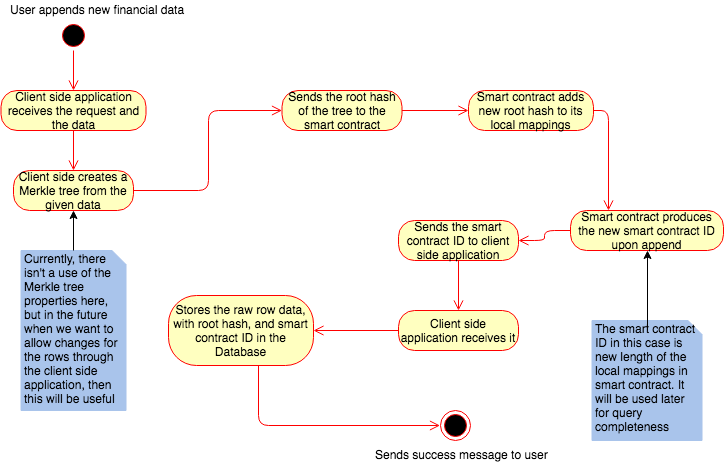
\includegraphics[width=1.0\textwidth]{images/appendRowFinancials.png}
	\caption{\label{fig:appendRowFinancials}Activity diagram of appending a row to the financials record}
\end{figure}

\begin{enumerate}
	\item User appends a new financial data, providing all the required information to be in the database
	\item Client-side application then creates a Merkle tree from the given raw data
	\item Sends the root hash of the created Merkle tree to the smart contract
	\item Smart contract appends that new root hash into its local mappings.
	\item Smart contract increments the new length of the mapping, which is the smart contract ID that is going to be returned. This acts as an identifier to which hash belongs to which financial row. It is also used to preserve the ordering of the hashes which will later be used for query completeness.
	\item Smart contract sends back the smart contract ID to the client-side application
	\item Client-side application saves the raw financial data, with the root hash, and the smart contract ID in the database. (See also Table \ref{table:recordsOffChain} to see how records are saved in the database)
\end{enumerate}

\subparagraph{Query Completeness Steps}
Below shows the implemented step by step actions when a user requests to perform query completeness. Figure \ref{fig:queryCompleteness} shows the activity diagram of the steps described below: 

\begin{figure}[h]
	\centering
	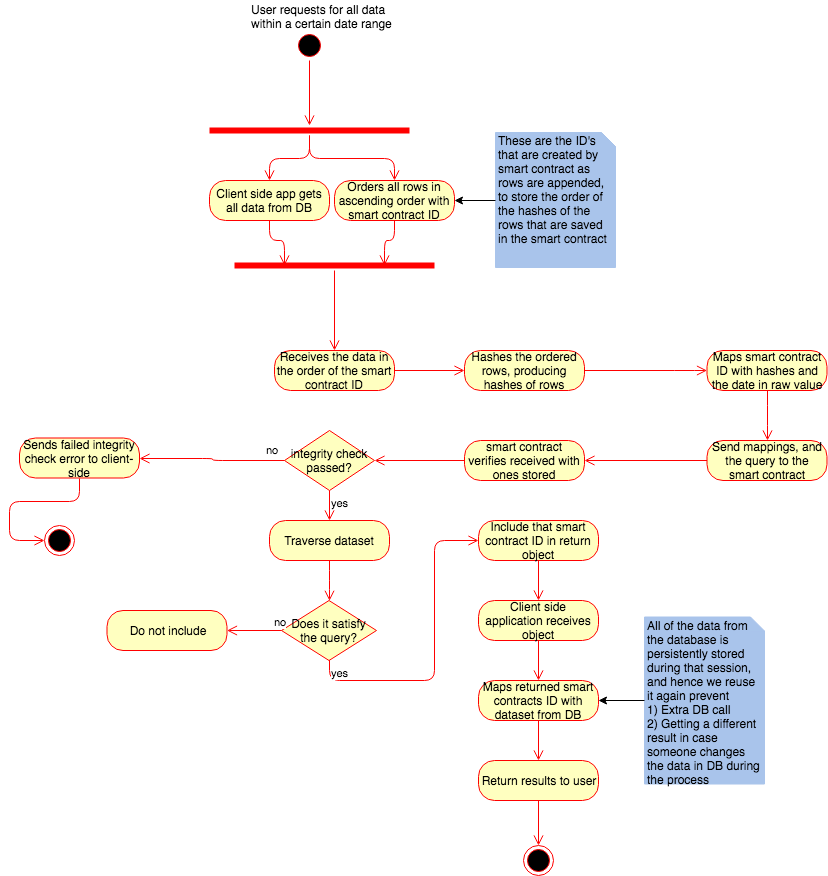
\includegraphics[width=1.0\textwidth]{images/queryCompleteness.png}
	\caption{\label{fig:queryCompleteness}Activity diagram for query completeness}
\end{figure}

\begin{enumerate}
	\item User requests to get all of financial data that are within the date range the user has requested.
	\item The client-side application gets all data from the database in the ascending order of the smart contract ID. This ID is generated by the smart contract to keep the ordering of the hashes that are stored in the smart contract. It is generated upon appending a financial record through the smart contract.
	\item The client-side application hashes each of the rows in the table.
	\item It will then map the hashes of the row and the raw date value to the smart contract ID.
	\item The client-side application sends the mapping with the query to the smart contract.
	\item The smart contract checks if it got the right data, the right amount of rows and the correct table overall by iterating over the provided root hashes and comparing them to the stored hashes in the local mapping.
		\begin{enumerate}
		\item If smart contract cannot verify the rows, then it will throw an integrity check error to the client-side application as an event.
		\item If the smart contract can confirm this, it checks the query condition for every row and returns an array of booleans indicating all the indexes of rows that fulfill the query. Dates are intentionally stored as “uint” to ease the query function in the smart contract. For example 1, March, 2018 -> 20180301
		\end{enumerate}
	\item Smart contract triggers an event to return back all the smart contract IDs that have satisfied the query.
	\item The client-side application listens to this event and returns the specified rows to the user subsequently.
\end{enumerate}

